\chapter{Stabilità nei sistemi dinamici}


\section{Definizione sistema dinamico e punti di equilibrio}

Un sistema dinamico 
è composta da uno stato \(x \in \mathbb{R}^{n}\)
e da una legge di evoluzione
\[\dot{x}(t) = f(x(t), u(t), t)\]


\begin{definition}
Un sistema è detto \textbf{tempo invariante} se la
  sua evoluzione non dipende esplicitamente dal tempo \(t\), cioè:
  \[\dot{x}(t) = f(x(t), u(t))\]
\end{definition}


\begin{definition}
Un sistema è detto \textbf{autonomo} se la sua evoluzione non dipende esplicitamente
  dall'ingresso \(u(t)\), cioè:
  \[\dot{x}(t) = f(x(t),t)\]
\end{definition}


Se il sistema è sia autonomo che tempo invariante
allora si ha:
\[\dot{x}(t) = f(x(t))\]




\begin{definition}
Dato un sistema dinamico \textbf{tempo invariante} nella forma:
\[\dot{x}(t) = f(x(t), u(t))\]
un punto di equilibrio \((\bar{x}, \bar{u})\) è una coppia 
stato-ingresso tale che:
\[\dot{x} = f(\bar{x}, \bar{u}) = 0\]


\end{definition}



\section{Definizione stabilità}

Un sistema dinamico 
tempo invariante è detto stabile se 

\[\forall \varepsilon > 0, 
\exists \delta > 0 : x_{0} 
\in B_{\delta}(\bar{x})
\Rightarrow |x_{x_{0}}(t) - \bar{x}| \le \varepsilon, \forall t \geq 0\]

Dove con \(x_{x_{0}}(t)\) si intende 
la traiettoria del sistema 
che parte da \(x_{0}\).


Ora dimostriamo che \(\delta \le 
\varepsilon ,
\forall \varepsilon > 0\).
Supponiamo per assurdo che 
esista un \(\varepsilon >0 \)
per cui si ha  
che la \(\delta\)
per cui è rispettata la 
definizione di stabilità sia
tale che
\(\delta > \varepsilon\).
Allora si ha che per
le 
\(x_{0} \in B_{\delta}(\bar{x}) \backslash
B_{\varepsilon}(\bar{x})\)
vale:
\[|x_{x_{0}}(0) - \bar{x}| 
= \left|x_{0} -\bar{x}\right|> \varepsilon\]
Ma questo è assurdo perché
\(x_{0} 
\in B_{\delta}(\bar{x})\)
dunque rispetta la definizione 
di stabilità per cui
si dovrebbe avere :
\[|x_{x_{0}}(0) - \bar{x}| 
= \left|x_{0} - \bar{x}\right|
\le \varepsilon
\]
Dunque siamo arrivati ad un assurdo.

% ...existing code...
\begin{figure}[h]
  \centering
  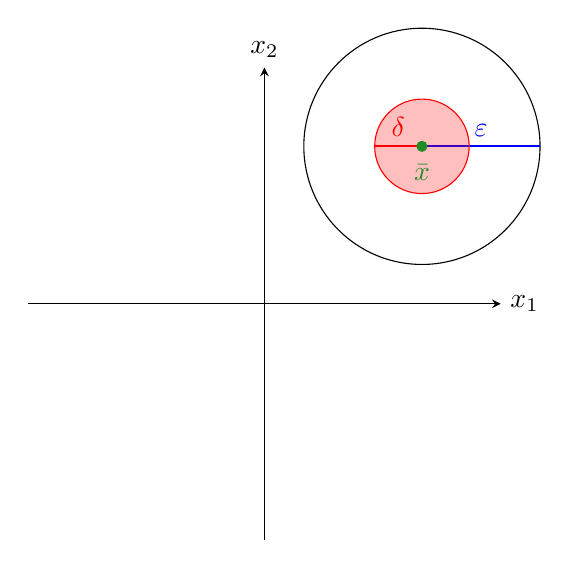
\begin{tikzpicture}[scale=1, >=stealth]
    % assi con sole etichette x1 e x2
    \draw[->] (-3,0) -- (3,0) node[right] {$x_1$};
    \draw[->] (0,-3) -- (0,3) node[above] {$x_2$};


    % cerchio grande e raggio epsilon
    \draw (2,2) circle (1.5);
    \draw[thick, blue] (2,2) -- ++(1.5,0) node[midway, above] {$\varepsilon$};

    % cerchio piu' piccolo rosso trasparente e raggio delta (più corto)
    \filldraw[fill=red, fill opacity=0.25, draw=red] (2,2) circle (0.6);
    \draw[thick, red] (2,2) -- ++(-0.6,-0) node[midway, above] {$\delta$};

    \filldraw[ForestGreen] (2,2) circle (1.8pt) node[below=3pt] {$\bar{x}$};

  \end{tikzpicture}
  \caption{In \textcolor{ForestGreen}{verde} si ha il 
  punto di equilibrio \textcolor{ForestGreen}{\(\bar{x}\)}. 
  In rosso si ha l'insieme delle condizioni iniziali per cui le traiettorie rimangono
  confinate  all'interno del cerchio di raggio \(\varepsilon\).}
  \label{fig:assi-x1-x2}
\end{figure}
% ...existing code...
\section{Stabilità nei sistemi lineari}

Consideriamo un sistema lineare
tempo invariante:
\[\dot{x}(t) = Ax(t) + Bu(t)\]
Dove \(A \in \mathbb{R}^{n \times n}\) e 
\(B \in \mathbb{R}^{n \times m}\).
Per trovare i punti di equilibrio dobbiamo imporre:
\[\dot{x}(t) = 0 \Longleftrightarrow Ax(t) + Bu(t) = 0\]
Dunque i punti di equilibrio 
sono i punti \((\bar{x}, \bar{u})\)che soddisfano:
\[ 
A\bar{x} + B\bar{u} = 0
\]

Notiamo subito che il punto \((\bar{x}, \bar{u}) = (0,0)\) è sicuro un punto di equilibrio.

